\section{Theorie}
\subsection{Das Sagnac-Interferometer}
Der schematische Aufbau eines Sagnac-Interferometers ist in Abbildung $\ref{aufbauschema}$ dargestellt.
Der von der Lichtquelle stammende Strahl trifft über zwei, zur Strahljustierung genutzte,
Spiegel auf einen PBSC. PBSC steht hierbei für  Polarizing-Beam-Splitter-Cube. Dieser besteht aus zwei Prismen, welche durch ein
Dielektrikum verbunden wurden. Der PBSC teilt den Strahl in zwei senkrecht zueinander
polarisierte Strahlen, welche orthogonal voneinander aus diesem austreten. Durch drei weitere justierbare Spiegel werden die beiden Strahlen auf eine Bahn gebracht, die sie in entgegengesetzter Richtung durchlaufen
und welche sie zurück zum PBSC führt. Von dort aus überlagern sich die beiden Teilstrahlen und werden auf einen zweiten, um 45° geneigten, PBSC gelenkt, der diese erneut trennt
und auf zwei verschiedene Photodioden bricht.
\begin{figure}[H]
  \centering
  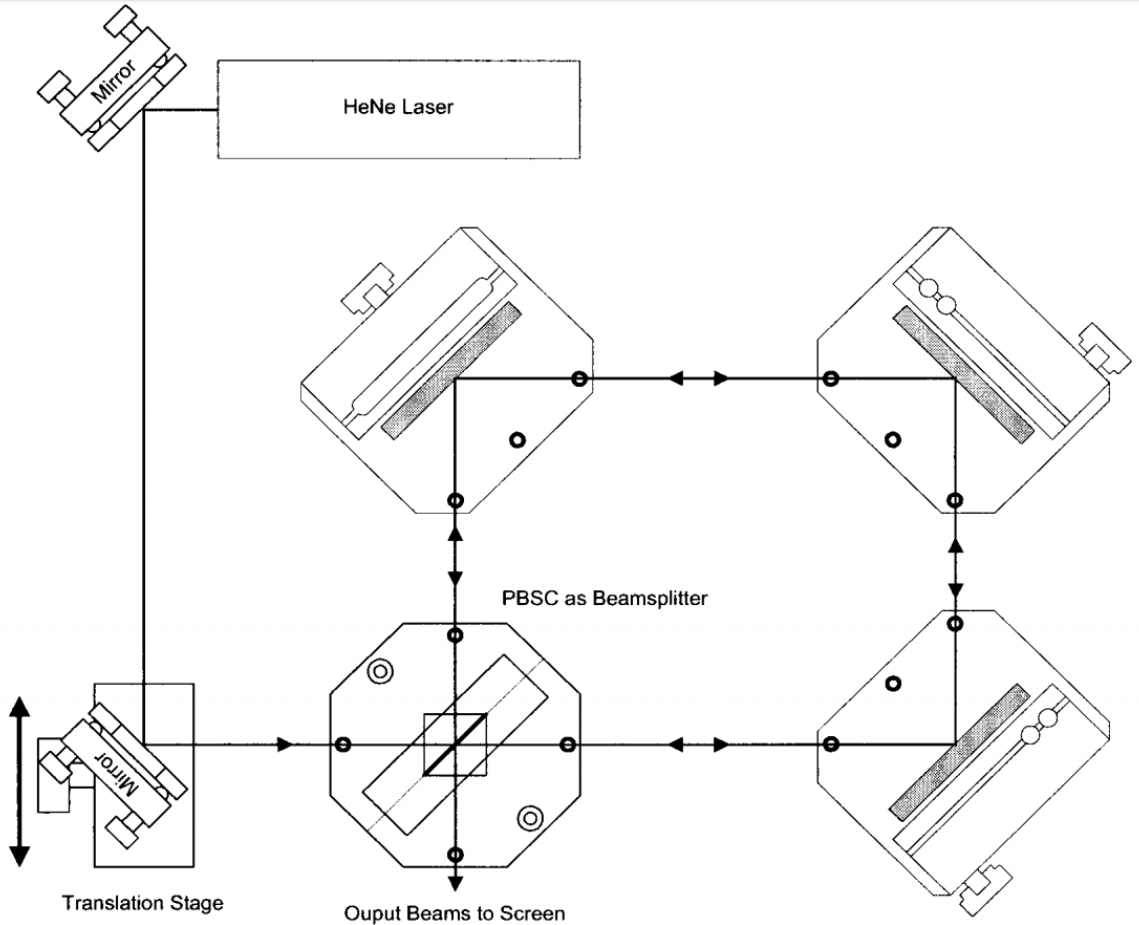
\includegraphics[scale=0.4]{Bilder/schema.png}
  \caption{Schematische Darstellung eines Sagnac-Interferometers.\cite{anleitung}}
  \label{aufbauschema}
\end{figure}
Die geringe Störungsempfindlichkeit des Sagnac-Interferometers stammt also daher, dass beide Teilstrahlen denselben Umweltfaktoren ausgesetzt sind.
\subsection{Kontrast eines Interferometers}
Der Kontrast eines Interferometers wird über die  Differenz zwischen der höchsten und der niedrigsten gemessenen Lichtintensität definiert. Es gilt
\begin{equation}
  K=\frac{I_{\text{max}}-I_{\text{min}}}{I_{\text{max}}+I_{\text{min}}}.
  \label{eq:kontrast}
\end{equation}
Bei einer perfekten absoluten Auslöschung wäre also ein Kontrast von 1 zu erreichen. Für das Sagnac-Interferometer wird der Kontrast über einen Polarisationfilter, welcher vor dem ersten PBSC platziert
wird, optimiert. Zur Herleitung des mathematischen Zusammenhangs zwischen Polarisationswinkel $\phi$ und Kontrast muss zunächst die Winkelabhängigkeit der Intensität bestimmt werden.
Für diese gilt
\begin{equation}
I \propto \left<\left|E_1\cos{(\phi)}\cos{(\omega t)}+E_2\sin{(\phi)}\cos{(\omega t+\delta)}\right|^2\right> ,
\end{equation}
wobei $\left<......\right>$ eine zeitliche Mittelung über eine Periode darstellt und $E_i$ die Amplitude des elektrischen Felds der jeweiligen Lichtstrahlen bezeichnet.
Es lässt sich feststellen, dass:
\begin{equation}
  \left<\cos^2(\omega t +\delta)\right> = \frac{1}{2} \nonumber
\end{equation}
\begin{equation}
  \delta_{\text{destruktiv}}=2\pi  \nonumber
\end{equation}
\begin{equation}
  \delta_{\text{konstruktiv}}=2\pi n + \pi \nonumber ,
\end{equation}
wobei $n$ eine natürliche ganze Zahl ist. Es folgt somit für $I_{\text{max}/\text{min}}$
\begin{equation}
  I_{\text{max}/\text{min}} \propto I_{\text{Laser}}\left(1 \pm 2\cos(\phi)\sin(\phi)\right).
\end{equation}
Hiermit folgt für die Polarisationswinkelabhängigkeit des Kontrasts
\begin{equation}
  K(\phi)=\sin(2\phi).
\end{equation}
Es ist somit leicht zu erkennen, dass der höchste Kontrast bei einem Polarisationswinkel von $45°$ auftreten sollte.
\subsection{Brechungsindexbestimmung von Gasen}
Die Bestimmung des Brechungsindexes von Gases basiert auf der Tatsache, dass für die Lichtgeschwindigkeit in einem Medium mit Brechungsindex $n$ gilt:
\begin{equation}
  v=\frac{c}{n}
\end{equation}
Die Veränderung der Ausbreitungsgeschwindigkeit des Lichts beeinflusst den Wellenvektor gemäß
\begin{equation}
  k = \frac{2\pi}{\lambda_{\text{vac}}}n.
\end{equation}
Hierbei bezeichnet $\lambda_{\text{vac}}$ die Vakuumwellenlänge.
Aus diesem Grund erfährt ein Strahl, welcher in ein Medium mit einem veränderten Brechungsindex eintritt, eine Phasenverschiebung gemäß:
\begin{equation}
  \Delta \phi= \frac{2\pi}{\lambda_{\text{vac}}}(n-1)L \, ,
  \label{eq:sieben}
\end{equation}
wobei  $L$ die in dem Medium durchquerte Strecke bezeichnet. Die entstandene Phasenverschiebung kann beim Sagnac-Interferometer zu Interferenzeffekten führen. Es lässt sich also
aus der Anzahl der gemessen Maxima der Brechungindex ermitteln. Für die Maxima gilt
\begin{equation}
  M = \frac{\Delta \phi}{2 \pi}.
\end{equation}
Über $\ref{eq:sieben}$ ist es möglich, den Brechungsindex aus der Anzahl der Maxima zu bestimmen:
\begin{equation}
  n=\frac{M\lambda_{\text{vac}}}{L}+1
\end{equation}
\subsection{Brechungsindexbestimmung von Glas}
Ähnlich wie bei der Bestimmung des Brechungsindexes von Gasen, wird auch bei Glas die Anzahl der auftretenden Interferenzmaxima genutzt, um $n$ zu berechnen. Beim Sagnac-Interferometer
werden hierbei die beiden entgegengesetzt laufenden Strahlen jeweils durch ein, um den Winkel $\theta$ geneigtes, Glasplättchen geleitet. Beim Durchqueren
der Glasplättchen treten zwei phasenverschiebende Effekte auf; zum einen wird durch die geometrische Lichtbrechung die Phase verschoben und zum anderen tritt wie beim
Gas eine Phasenverschiebung durch den Brechungsindex direkt auf.
Die Anzahl der Interferenzmaxima, welche durch diese, kompliziert zu berechnende, Phasenverschiebung auftritt, lässt  sich mit
\begin{equation}
  M \approx \frac{2T}{\lambda_{\text{vac}}}\frac{n-1}{2n}\theta^2
\end{equation}
annähern. Hierbei bezeichnet $T$ die Dicke der Platten. Somit folgt für den Brechungsindex
\begin{equation}
  n=1-\frac{T\theta^2}{M\lambda_{\text{vac}}}.
\end{equation}
